%!TEX program = xelatex

% \documentclass[10pt]{article}
%%%%%%%%%%%%%%%%%%%%%%%%%%%%%%%%%%%%%%%%%
% Modified By Orcuslc, 2016-9-21
% Modified for Assignments
% http://github.com/orcuslc
%
% Wilson Resume/CV
% Structure Specification File
% Version 1.0 (22/1/2015)
%
% This file has been downloaded from:
% http://www.LaTeXTemplates.com
%
% License:
% CC BY-NC-SA 3.0 (http://creativecommons.org/licenses/by-nc-sa/3.0/)
%
%%%%%%%%%%%%%%%%%%%%%%%%%%%%%%%%%%%%%%%%%

%----------------------------------------------------------------------------------------
%	PACKAGES AND OTHER DOCUMENT CONFIGURATIONS
%----------------------------------------------------------------------------------------
\documentclass[10pt]{article}

\usepackage{listings}
\usepackage{xcolor}
\usepackage{amsmath,amsthm,amssymb}
\usepackage{epstopdf}
\usepackage{graphicx}
\usepackage{clrscode3e}

\DeclareGraphicsExtensions{.eps,.ps,.jpg,.bmp}


\usepackage[a4paper, hmargin=25mm, vmargin=30mm, top=20mm]{geometry} % Use A4 paper and set margins

\usepackage{fancyhdr} % Customize the header and footer

\usepackage{lastpage} % Required for calculating the number of pages in the document

\usepackage{hyperref} % Colors for links, text and headings

\setcounter{secnumdepth}{0} % Suppress section numbering

%\usepackage[proportional,scaled=1.064]{erewhon} % Use the Erewhon font
%\usepackage[erewhon,vvarbb,bigdelims]{newtxmath} % Use the Erewhon font
\usepackage[utf8]{inputenc} % Required for inputting international characters
\usepackage[T1]{fontenc} % Output font encoding for international characters

\usepackage{fontspec} % Required for specification of custom fonts
\setmainfont[Path = ./fonts/,
Extension = .otf,
BoldFont = Erewhon-Bold,
ItalicFont = Erewhon-Italic,
BoldItalicFont = Erewhon-BoldItalic,
SmallCapsFeatures = {Letters = SmallCaps}
]{Erewhon-Regular}

\usepackage{color} % Required for custom colors
\definecolor{slateblue}{rgb}{0.17,0.22,0.34}

\usepackage{sectsty} % Allows customization of titles
\sectionfont{\color{slateblue}} % Color section titles

\fancypagestyle{plain}{\fancyhf{}\cfoot{\thepage\ of \pageref{LastPage}}} % Define a custom page style
\pagestyle{plain} % Use the custom page style through the document
\renewcommand{\headrulewidth}{0pt} % Disable the default header rule
\renewcommand{\footrulewidth}{0pt} % Disable the default footer rule

\setlength\parindent{0pt} % Stop paragraph indentation

% Non-indenting itemize
\newenvironment{itemize-noindent}
{\setlength{\leftmargini}{0em}\begin{itemize}}
{\end{itemize}}

% Text width for tabbing environments
\newlength{\smallertextwidth}
\setlength{\smallertextwidth}{\textwidth}
\addtolength{\smallertextwidth}{-2cm}

\newcommand{\sqbullet}{~\vrule height .8ex width .6ex depth -.05ex} % Custom square bullet point 


\newcommand{\tbf}[1]{\textbf{#1}}
\newcommand{\tit}[1]{\textit{#1}}
\newcommand{\mbb}[1]{\mathbb{#1}}
\newcommand{\blue}[1]{\color{blue}{#1}}
\newcommand{\red}[1]{\color{red}{#1}}
\newcommand{\sblue}[1]{\color{slateblue}{#1}}
\newcommand{\n}{\\[5pt]}
\newcommand{\tr}{^\top}
\newcommand{\vt}[1]{
\Vert #1 \Vert
}
\newcommand{\bra}[5]{
#1=\left\{
\begin{aligned}
#2 ,&\quad #4 \\
#3 ,&\quad #5
\end{aligned}
\right.
}

\renewcommand{\title}[2] {
{\Huge{\color{slateblue}\textbf{#1}}}
\hfill
\LARGE{\color{slateblue}\textbf{#2}} \\[10pt]
\large{\color{slateblue}\textbf{Chuan Lu, 13300180056, chuanlu13@fudan.edu.cn}} \\[1mm]
\rule{\textwidth}{0.5mm}
}

\newcommand{\problem}[2] {
\vspace{20pt}
\LARGE{\color{slateblue}\textbf{Problem #1.}}
\vspace{2mm}
#2 \\[10pt]
}

\renewcommand{\proof}[2] {
\large{\color{slateblue}\textit{\textbf{#1.}}}
#2 \qed \\[3mm]
}

\newcommand{\solution}[2] {
\large{\color{slateblue}\textit{\textbf{#1.}}}
#2 \\[3mm]
}


\newcommand{\algorithm}[2] {
\begin{codebox}
\Procname{$\proc{Algorithm #1}$}
#2
\end{codebox}
}

\newcommand{\refgroup}[1] {
\LARGE{\color{slateblue}\textbf{Reference}} 
\begin{tabbing}
\hspace{5mm} \= \kill
#1
\end{tabbing}
}

\newcommand{\reference}[1] {
\sqbullet \ \  \large{#1} \\
}
% \newcommand{\solution}[2] {
% \LARGE{\color{slateblue}\textit{#1}}
% \ #2 \qed
% }

% \newenvironment{problem}[2][Problem]{\begin{trivlist}
% \item[\hskip \labelsep {\bfseries #1}\hskip \labelsep {\bfseries #2.}]}{\end{trivlist}}
\usepackage{epstopdf}
\usepackage{graphics}
\usepackage{subfig}
\usepackage{listings}
\lstset{
  numbers=left,
    framexleftmargin=10mm,
    frame=none,
    backgroundcolor=\color[RGB]{245,245,244},
  keywordstyle=\bf\color{blue},
  identifierstyle=\bf,
  numberstyle=\color[RGB]{0,192,192},
  commentstyle=\it\color[RGB]{0,96,96},
  stringstyle=\rmfamily\slshape\color[RGB]{128,0,0},
  showstringspaces=false,
  extendedchars=false
    }
\DeclareGraphicsExtensions{.eps,.ps,.jpg,.bmp}

\begin{document}

\title{Homework 3}{16.11.4}

% \parbox{0.3\textwidth}{
% Chuan Lu}
% \hfill
% \parbox{0.3\textwidth}{
% 13300180056}
% \hfill
% \parbox{0.3\textwidth}{
% chuanlu13@fudan.edu.cn}

\problem{1}{Perform PCA to assign31.csv.}
\solution{Result}{
Since there are many NAs in assign31.csv, we changed those NA to 0. \n
The results are as follows: The rate in the table is the rate of information reserved after PCA.
\begin{table}[htbp] \large \centering
\begin{tabular}{|c|c|c|c|c|c|c|}
\hline
k & 1 & 2 & 3 & 5 & 10 & 14  \\
\hline
Rate & 0.2139058 &  0.396026 & 0.5165856 & 0.6697862 & 0.920202 & 1\\
\hline
\end{tabular}
\caption{Reserved information rate of different orders in PCA.}
\end{table}

\begin{figure}[htbp]
\centering
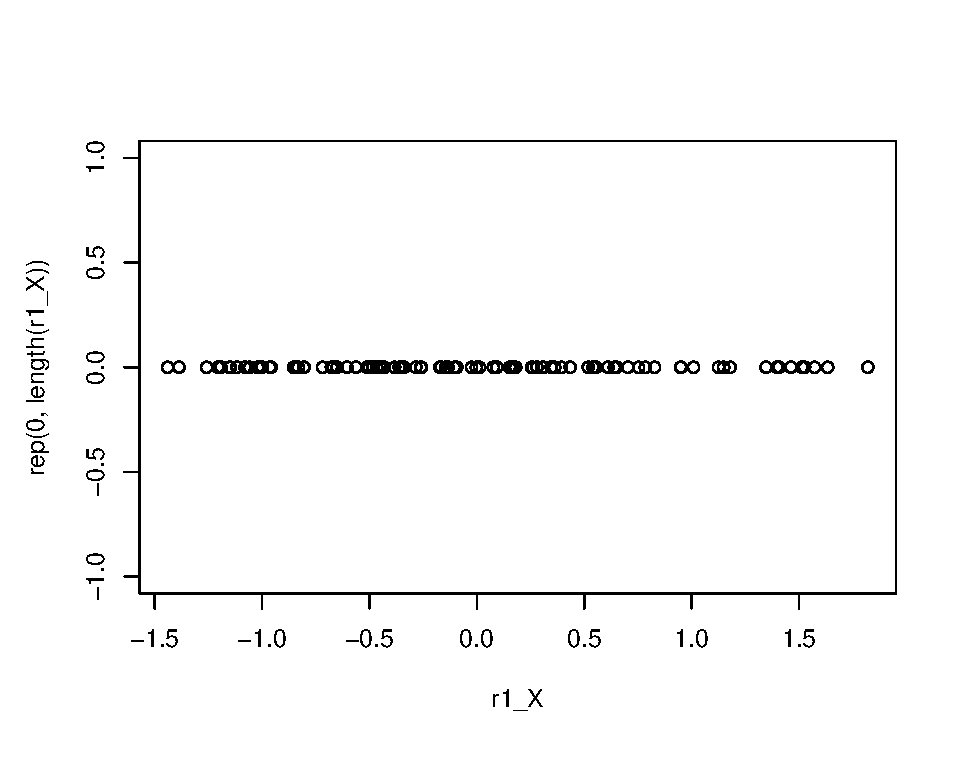
\includegraphics[width = 15cm]{pics/hw1_pca_1.eps}
\caption{PCA, k = 1}
\label{PCA1}
\end{figure}
\begin{figure}[htbp]
\centering
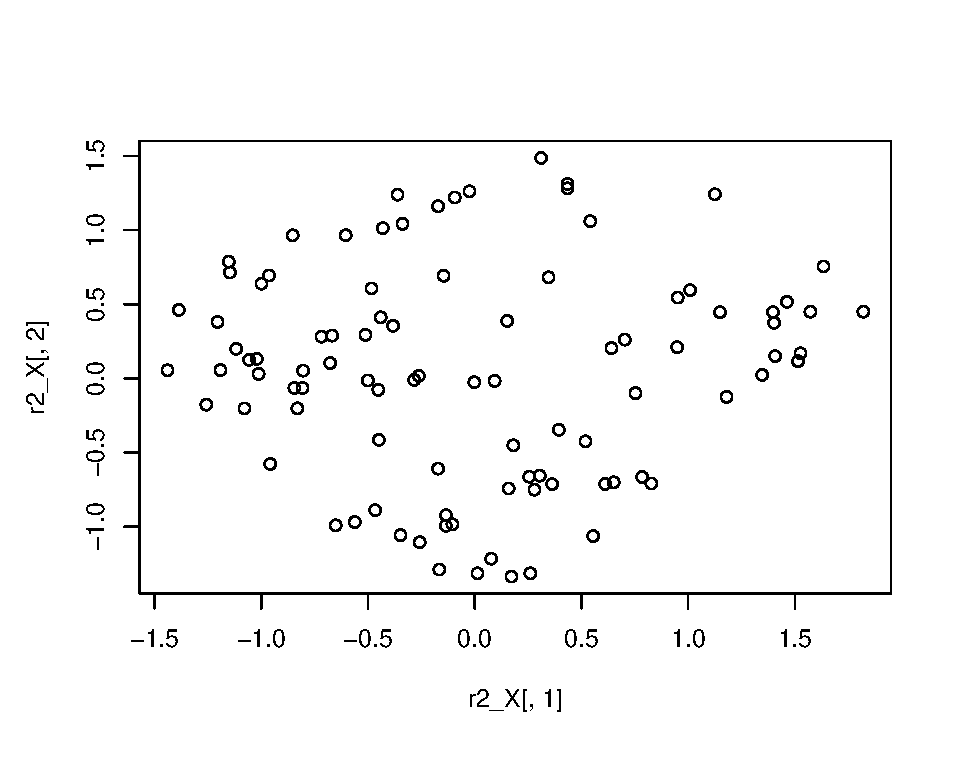
\includegraphics[width = 15cm]{pics/hw1_pca_2.eps}
\caption{PCA, k = 2}
\label{PCA2}
\end{figure}
\begin{figure}[htbp]
\centering
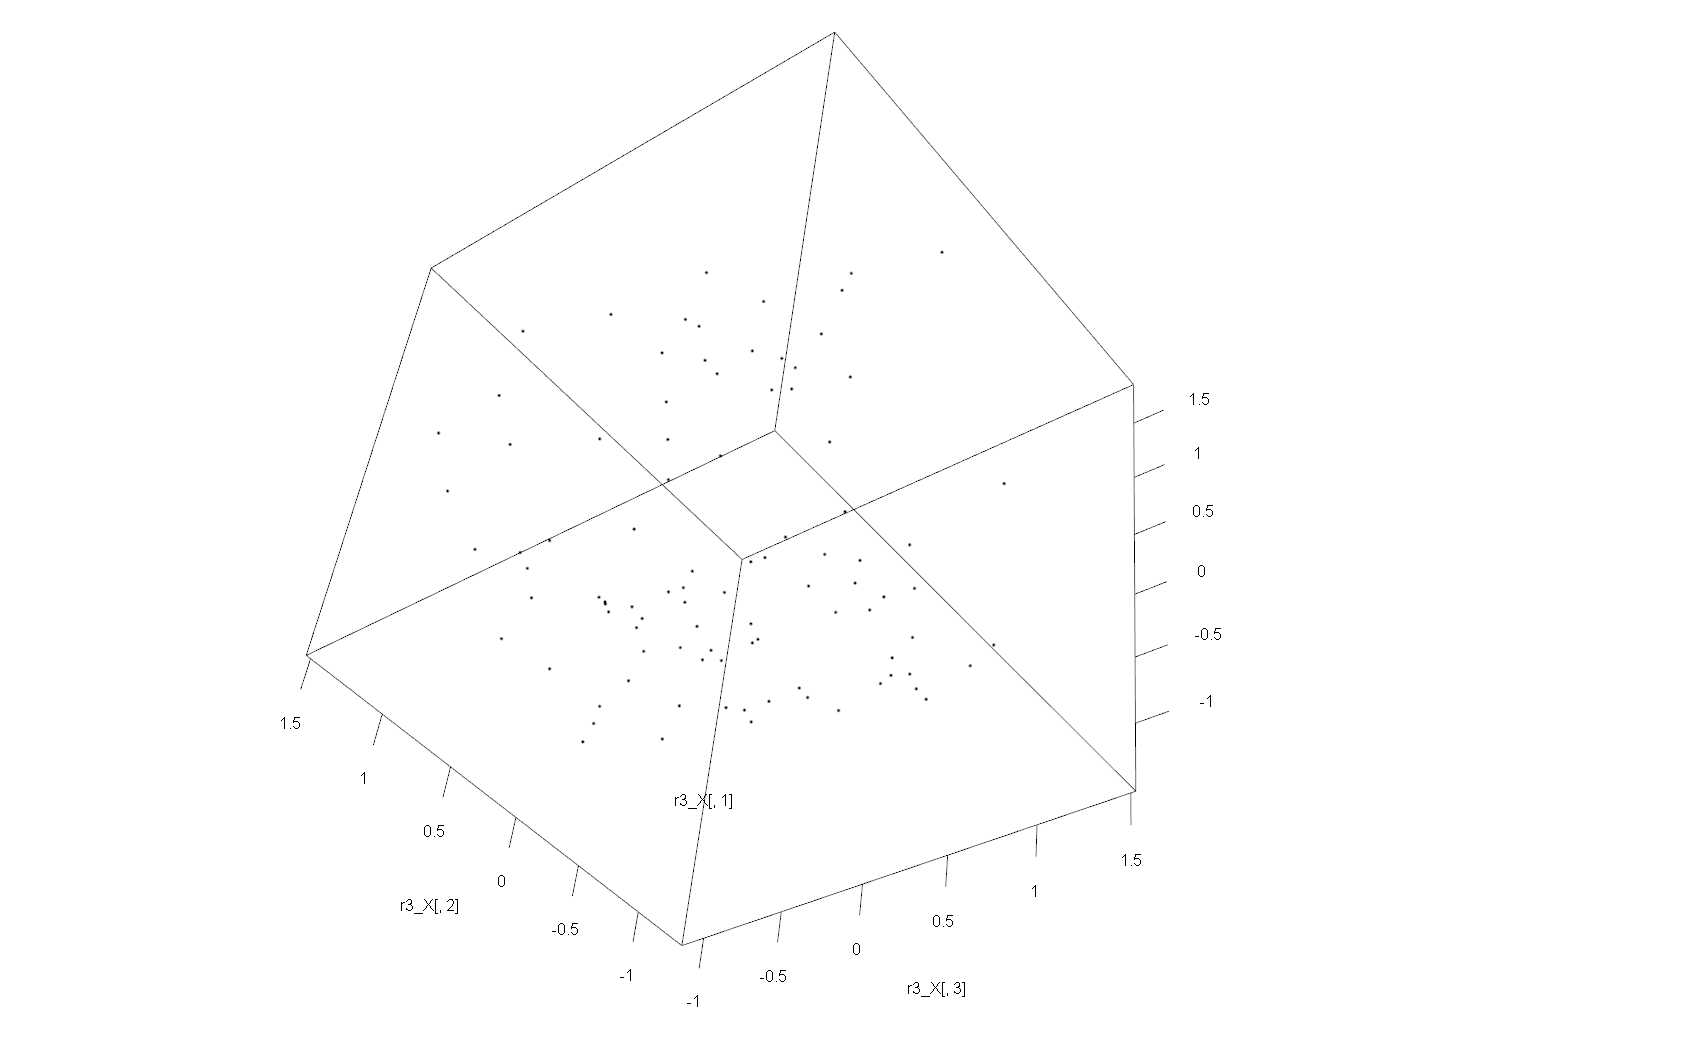
\includegraphics[width = 15cm]{pics/hw1_pca_3.png}
\caption{PCA, k = 3}
\label{PCA3}
\end{figure}
From these figures(when $k = 1, 2, 3$) we can find that after PCA the data points still seem to be random and messy. When we calculate the rate of reserved information we can know that not until $k = 10$ the rate is less than 0.9, which is thought to be unsatisfying.
}


\problem{2}{Perform PCA and NMF to assign2.csv, and explain the difference.}
\solution{Result}{
For PCA, the result is as follows:
\begin{table}[htbp] \large \centering
\begin{tabular}{|c|c|c|c|}
\hline
k & 1 & 2 & 3  \\
\hline
Rate & 0.4326317 &  0.7648243 & 0.9298461 \\
\hline
\end{tabular}
\caption{Reserved information rate of different orders in PCA.}
\end{table}
\begin{figure}[htbp]
\centering
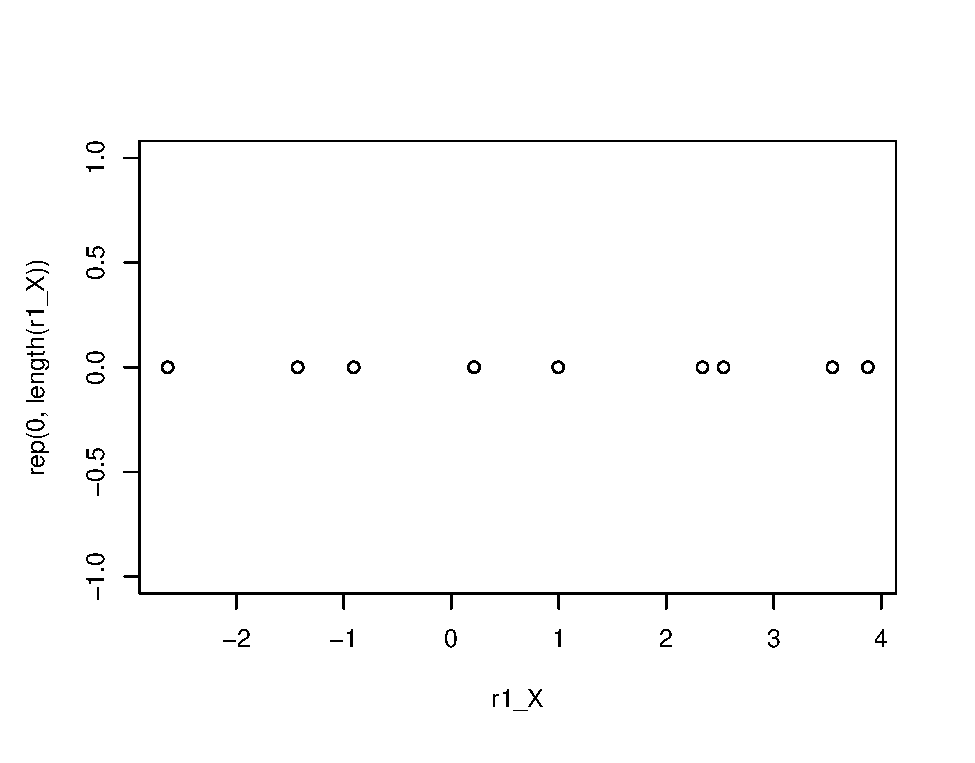
\includegraphics[width = 15cm]{pics/hw2_pca_1.eps}
\caption{PCA, k = 1}
\label{PCA1}
\end{figure}
\begin{figure}[htbp]
\centering
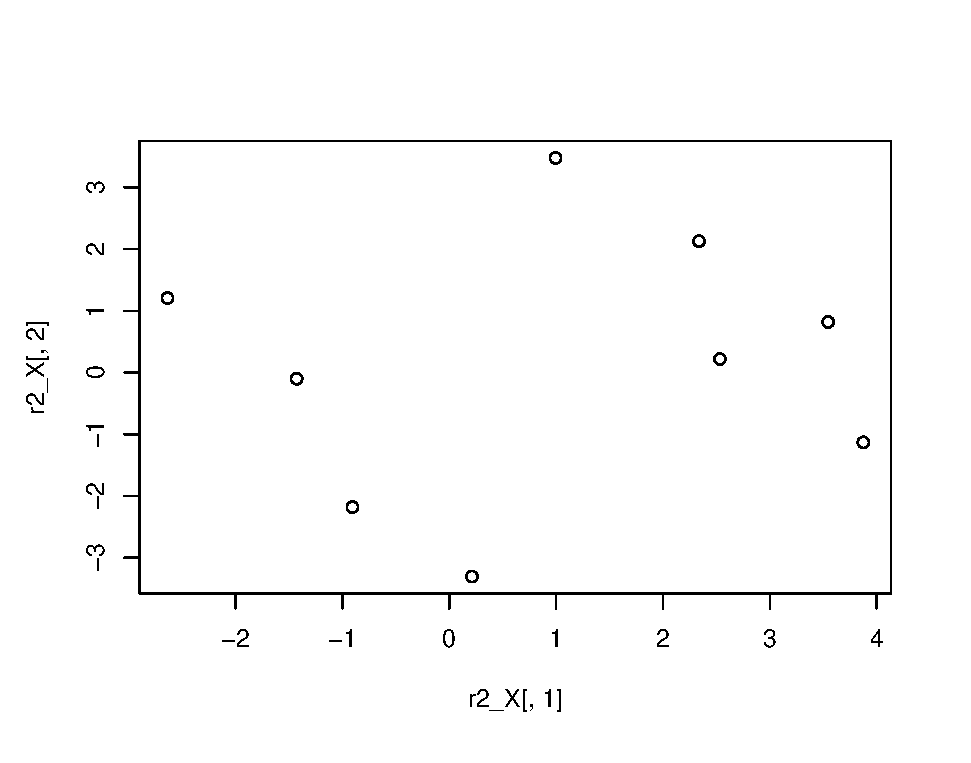
\includegraphics[width = 15cm]{pics/hw2_pca_2.eps}
\caption{PCA, k = 2}
\label{PCA2}
\end{figure}
\begin{figure}[htbp]
\centering
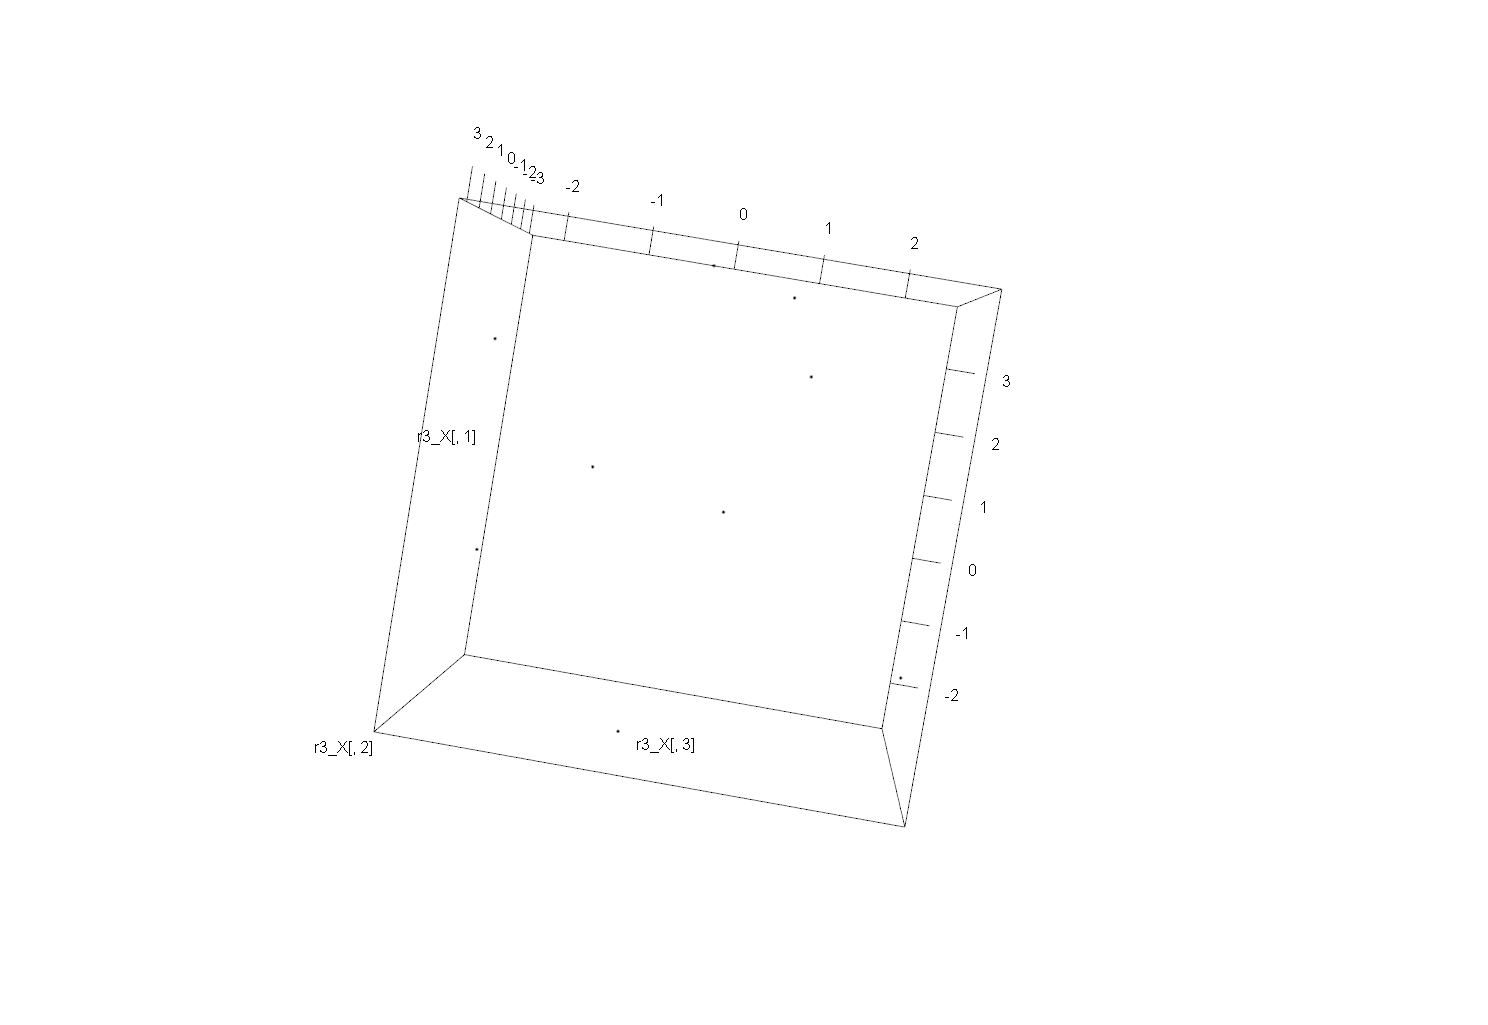
\includegraphics[width = 15cm]{pics/hw2_pca_3.png}
\caption{PCA, k = 3}
\label{PCA3}
\end{figure}
From figure(k = 1) we can assert nothing; from figure(k = 2) it seems the data can be simulated by two parallel lines. From the table we can find when k = 3, the rate of reserved information is over 0.9, which means k = 3 is a good estimation. \n
For NMF, the result of error rate is as follows:
$$ rate = \frac{\vt{A - WH}_F}{\vt{A}_F} $$
\begin{table}[htbp] \large \centering
\begin{tabular}{|c|c|c|c|c|c|}
\hline
k & 1 & 2 & 3 & 5 & 10\\
\hline
Rate & 0.6764784 &  0.6904373 & 2.629497 & 4.993591 & 14.36354\\
\hline
\end{tabular}
\caption{Error rates of different orders in NMF.}
\end{table}
It must be wrong somewhere that with k being larger, the estimation becoming worse. I think it should be the number of iterations, which is fixed at 1000.
}

\problem{3}{Perform PCA and nmf to test2.csv}
\solution{Result}{
For PCA, the result is shown as follows:
\begin{figure}[htbp]
\centering

\includegraphics[width = 5cm]{pics/hw3_original.png}
\caption{Original Picture}
\label{Original}
\end{figure}

\begin{figure}[htbp]
\centering
\subfloat[k = 1]{ %
	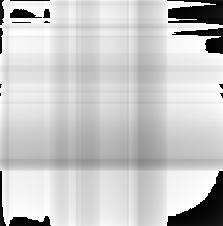
\includegraphics[width = 0.3\textwidth]{pics/hw3_pca_1.png}}\hfill
\subfloat[k = 2]{
	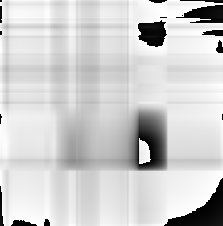
\includegraphics[width = 0.3\textwidth]{pics/hw3_pca_2.png}}\hfill
\subfloat[k = 3]{
	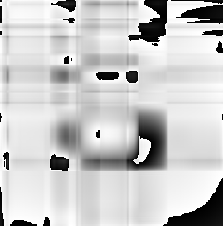
\includegraphics[width = 0.3\textwidth]{pics/hw3_pca_3.png}}	
\end{figure}
\begin{figure}[htbp]
\centering
\subfloat[k = 4]{ %
	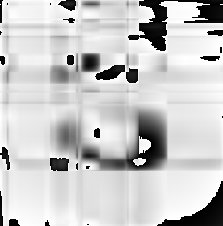
\includegraphics[width = 0.3\textwidth]{pics/hw4_pca_4.png}}\hfill
\subfloat[k = 5]{
	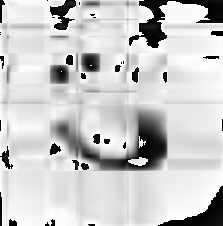
\includegraphics[width = 0.3\textwidth]{pics/hw3_pca_5.png}}\hfill
\subfloat[k = 10]{
	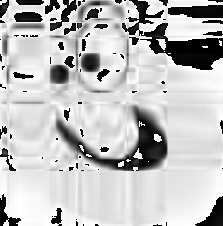
\includegraphics[width = 0.3\textwidth]{pics/hw3_pca_10.png}}	
\end{figure}
\begin{figure}[htbp]
\centering
\subfloat[k = 20]{ %
	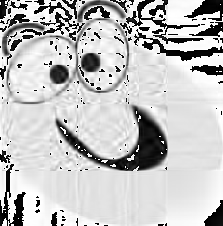
\includegraphics[width = 0.3\textwidth]{pics/hw3_pca_20.png}}\hfill
\subfloat[k = 50]{
	
\includegraphics[width = 0.3\textwidth]{pics/hw3_pca_50.png}}\hfill
\subfloat[k = 200]{
	
\includegraphics[width = 0.3\textwidth]{pics/hw3_pca_200.png}}	
\end{figure}
For NMF, 
}
\end{document}